\documentclass[12pt,a4paper]{article}
% Change "article" to "report" to get rid of page number on title page
\usepackage{amsmath,mathtools,amsfonts,amsthm,amssymb}
\usepackage{setspace}
\usepackage{Tabbing}
\usepackage{fancyhdr}
\usepackage{lastpage}
\usepackage{extramarks}
\usepackage{chngpage}
\usepackage{fourier}
\usepackage{soul,color}
\usepackage[usenames,dvipsnames]{xcolor}
\usepackage{graphicx,float,wrapfig}
\usepackage[utf8]{inputenc}
\usepackage{sidecap}
\usepackage{marvosym}
\usepackage{tikz, tikz-qtree}
\usepackage{tabularx, multirow}
\usepackage{enumerate}
\usepackage{hyperref}
\definecolor{gray99}{gray}{.99}
\usepackage{listings}
\usepackage[english]{babel}
\usepackage{placeins}
\usepackage{tikz}
\usepackage{tikz-qtree}
\usepackage{xspace}
\usepackage{mathtools}
\usepackage{tabulary}
\lstset{
	language=R,
	backgroundcolor=\color{gray99},
	tabsize=3,
	frame=single,
	keywordstyle=\ttfamily\bfseries\color{RoyalBlue},
	commentstyle=\ttfamily\color{ForestGreen},
	stringstyle=\ttfamily\color{Gray},
	breaklines=true,
	showstringspaces=false,
	basicstyle=\footnotesize\ttfamily,
	emph={label},
	xleftmargin=22pt,
	framexleftmargin=22pt,
	framexrightmargin=0pt,
	framexbottommargin=4pt,
	numbers=left,
	stepnumber=1
}
\usepackage{caption}
\DeclareCaptionFont{black}{\color{black}}{\bfseries}
\DeclareCaptionFormat{listing}{\parbox{\textwidth}{\hspace{8pt}#1#2#3}}
\captionsetup[lstlisting]{format=listing,labelfont=black,textfont=black, singlelinecheck=false, margin=0pt, font={bf,footnotesize}}

% In case you need to adjust margins:
\topmargin=-0.45in      %
\evensidemargin=0in     %
\oddsidemargin=0in      %
\textwidth=6.5in        %
\textheight=9.5in       %
\headsep=0.25in         %

% Special font
\newcommand{\cps}[2]{\ensuremath{[[{#1}]]_{\textstyle #2}}}

% Homework Specific Information
\newcommand{\hmwkTopic}{Predicting Crime Rates}
\newcommand{\hmwkTitle}{HW3 - \hmwkTopic}
\newcommand{\hmwkDueDate}{April 8, 2014}
\newcommand{\hmwkClass}{CS 199}
\newcommand{\hmwkAuthorNameA}{Sam Laane}
\newcommand{\hmwkAuthorEmailA}{laane2@illinois.edu}
\newcommand{\hmwkAuthorNameB}{José Vicente Ruiz}
\newcommand{\hmwkAuthorEmailB}{ruizcep2@illinois.edu}

% Setup the header and footer
\pagestyle{fancy}                                                       %
\lhead{\hmwkAuthorNameA \xspace \& \hmwkAuthorNameB}                                                 %
\chead{\hmwkClass}  %
\rhead{\hmwkTopic}     
                                                %
\lfoot{}                                                      %
\cfoot{\thepage}                                                        %
\rfoot{}                          %
\renewcommand\headrulewidth{0.4pt}                                      %
\renewcommand\footrulewidth{0.4pt}                                      %


%%%%%%%%%%%%%%%%%%%%%%%%%%%%%%%%%%%%%%%%%%%%%%%%%%%%%%%%%%%%%
% Make title
\title{\vspace{2in}\textmd{\hmwkClass\\\textbf{\hmwkTitle}}\\\normalsize\vspace{0.1in}\small{\hmwkDueDate}\\\vspace{4in}}
\date{}
\author{\textbf{\hmwkAuthorNameA} $\;$<\texttt{\href{mailto:laane2@illinois.edu}{\hmwkAuthorEmailA}}>\\\textbf{\hmwkAuthorNameB} $\;$<\texttt{\href{mailto:ruizcep2@illinois.edu}{\hmwkAuthorEmailB}}>}
%%%%%%%%%%%%%%%%%%%%%%%%%%%%%%%%%%%%%%%%%%%%%%%%%%%%%%%%%%%%%

\begin{document}
\begin{singlespace}

\begin{titlepage}
\maketitle
\thispagestyle{empty}
\end{titlepage}

% Uncomment the \tableofcontents and \newpage lines to get a Contents page
% Uncomment the \setcounter line as well if you do NOT want subsections
%       listed in Contents
%\setcounter{tocdepth}{1}
\tableofcontents
\newpage

% When problems are long, it may be desirable to put a \newpage or a
% \clearpage before each homeworkProblem environment

\clearpage

\section{Introduction}
This assignment consisted on the implementation of several \emph{regression} methods to try to predict the rate of violent crimes per population of several cities of the United States. \\

For that purpose, a dataset from the \emph{UC Irvine} machine learning repository was provided. The programming language used have been \texttt{R}, and this report have been typeset using \LaTeX.

\section{Removing variables with missing values}
\subsection{Implementation}
\lstinputlisting[firstline=13, lastline=23]{crimes.R}

\section{Basics - Linear regression}
\subsection{Implementation}
\lstinputlisting[firstline=31, lastline=79]{crimes.R}

\subsection{Results}

\begin{itemize}
	\item Mean-squared error on the \emph{whole data}: \textbf{1.66e-02}
  	\item Mean-squared error on the \emph{test data} (20\%): \textbf{1.88e-02}
  	\item Mean-squared error on the \emph{Box-Cox transformed data}: \textbf{1.85e-01}
\end{itemize}

\newpage
\subsubsection{Standard data}
\vspace{-0.5cm}
\begin{figure}[h!]
    \centering
    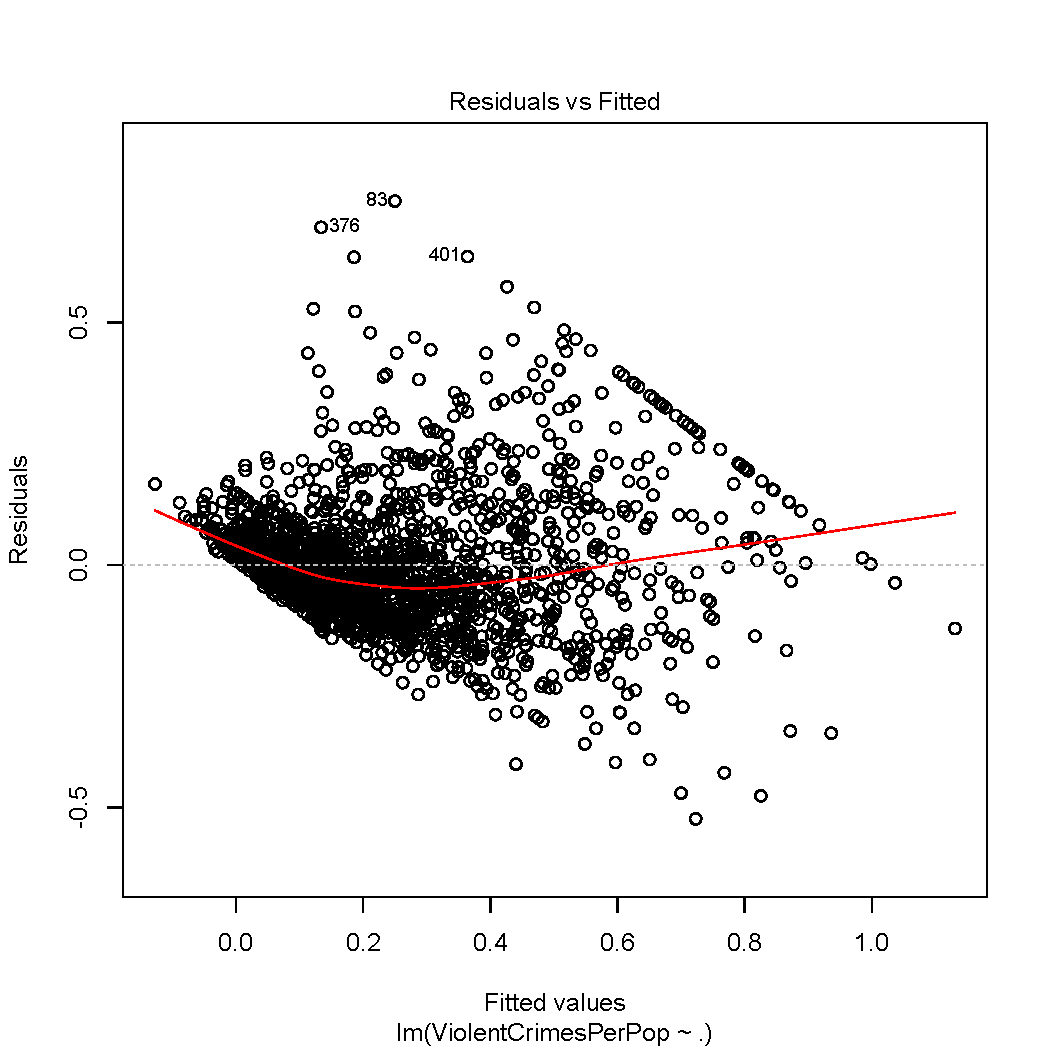
\includegraphics[width=0.7\textwidth,trim= 0 0 20 30, clip]{Linear_regression_residuals.pdf}
\end{figure}

\vspace{-0.5cm}
\begin{figure}[h!]
    \centering
    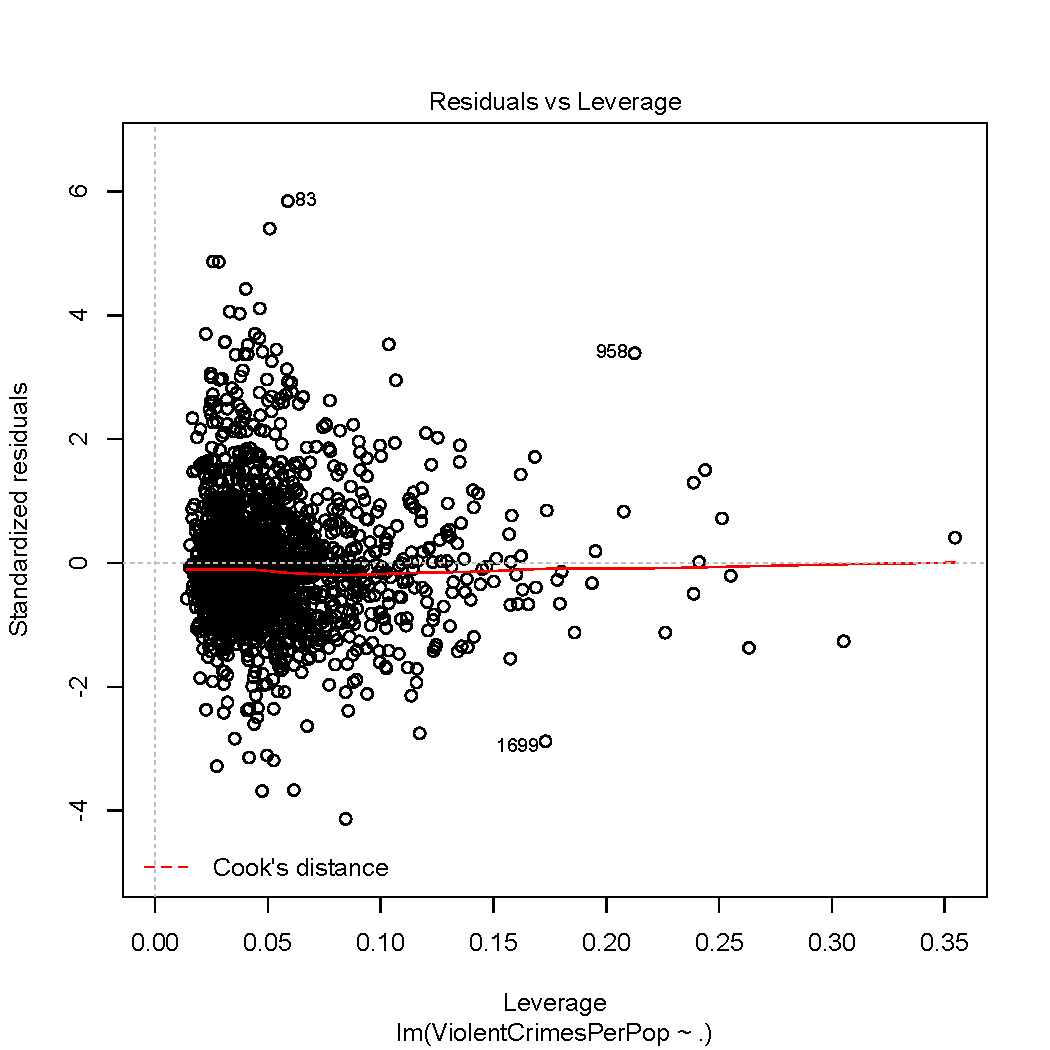
\includegraphics[width=0.7\textwidth,trim= 0 0 20 30, clip]{Linear_regression_cook.pdf}
\end{figure}
\FloatBarrier

\newpage
\subsubsection{Box-Cox transformed data}
\vspace{-0.5cm}
\begin{figure}[h!]
    \centering
    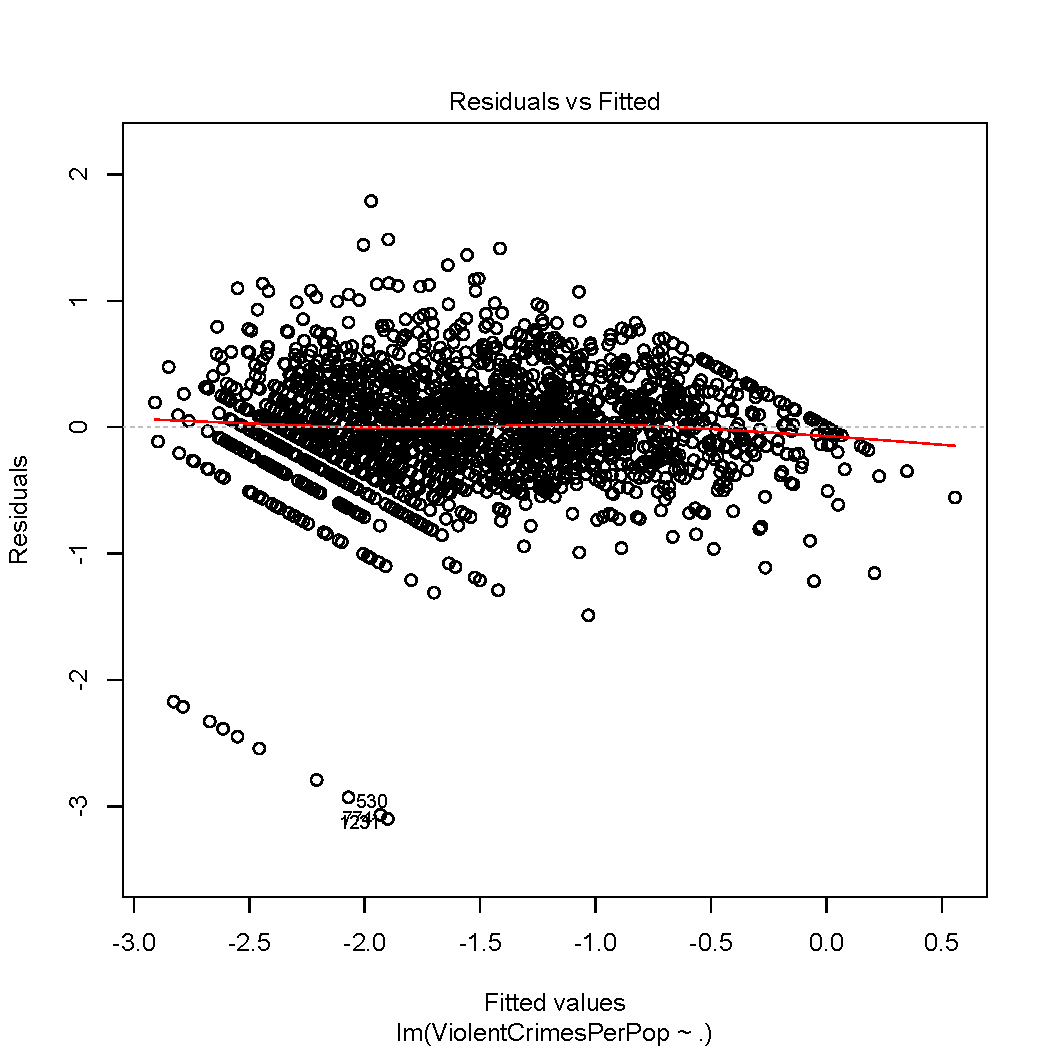
\includegraphics[width=0.7\textwidth,trim= 0 0 20 30, clip]{Boxcox_regression_residuals.pdf}
\end{figure}
\FloatBarrier

\vspace{-0.5cm}
\begin{figure}[h!]
    \centering
    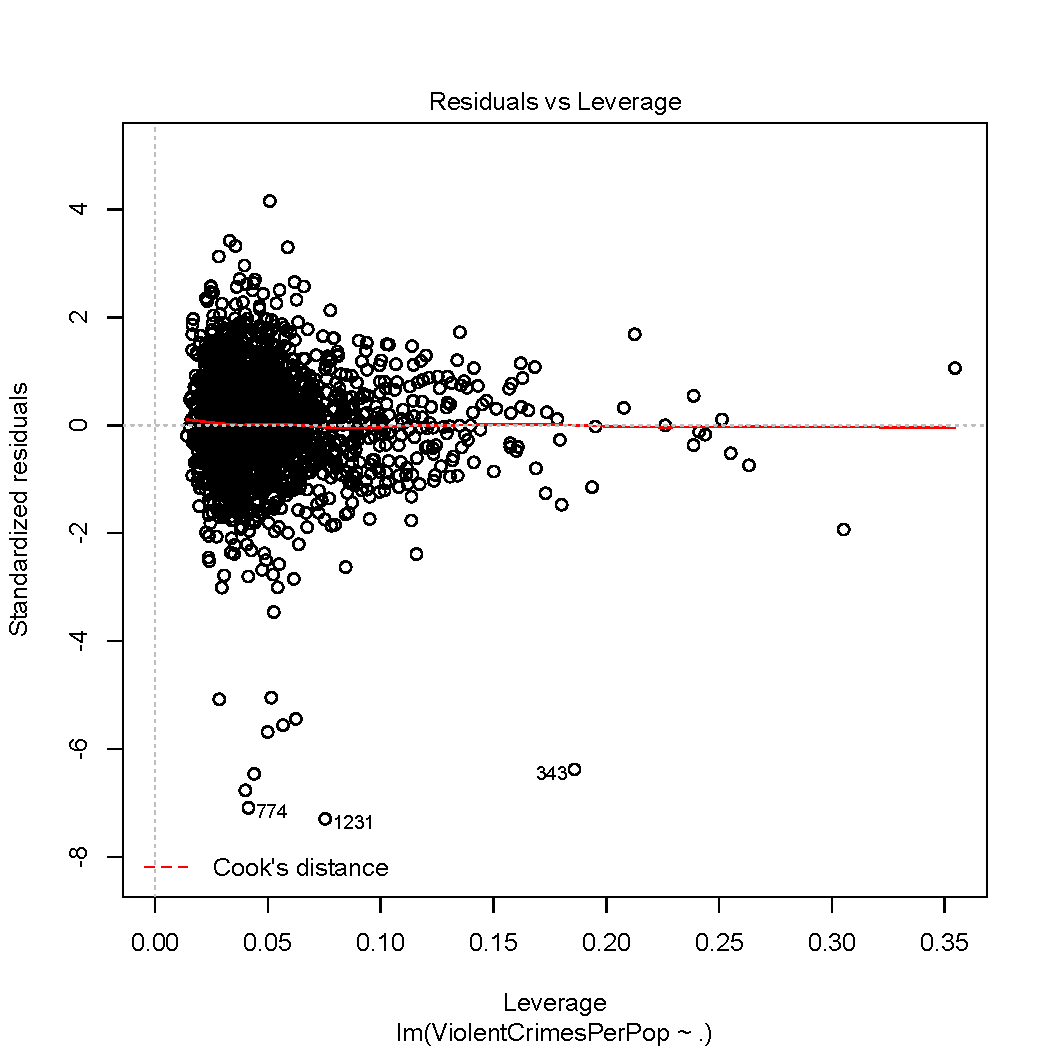
\includegraphics[width=0.7\textwidth,trim= 0 0 20 30, clip]{Boxcox_regression_cook.pdf}
\end{figure}
\FloatBarrier

\subsection{Conclusions}
\subsubsection{Standard data}
The Mean-squared error on both the full \emph{regression} and the \emph{regression} computed over the test data are both quite small. The later is a little larger probably because it has less data. \\

The residual graph was relatively poorly behaved with some strange linear structures.
The lack of a \emph{``banana''} shows that our problem is not likely to be fixed by \emph{Box-Cox} or other types of transformed. We need more explanatory values.
According to the \texttt{Residuals Vs Leverage} graph no points had undue influence
or we have to worry about \emph{Cook's distance}. This show that the \emph{regression} is likely possible with our data but needs work.


\subsubsection{Box-Cox transformed data}
The \emph{Box-Cox} transformed data looked promising but has a larger Mean-squared error. Besides, the residual graph shows that while the data looks straighter the linear structures can still be seen. \\

Moreover, when one accounts for the change in base of the distortion of the residual structure, the result looks far worse. We also see that at low fitted values the data looks split and some have extremely low residuals. This is likely caused by values extremely close to zero used to represent zero, which is required to generate the \emph{Box-Cox} transformation. So, in conclussion, \emph{Box-Cox} was useless. 

\section{Basics - Nearest Neighbor regression}
\subsection{Implementation}
\lstinputlisting[firstline=87, lastline=112]{crimes.R}

\subsection{Results}
\begin{itemize}
    \item Mean-squared error on the \emph{test data} (20\%): \textbf{3.64e-02}
\end{itemize}

\vspace{-0.5cm}
\begin{figure}[h!]
    \centering
    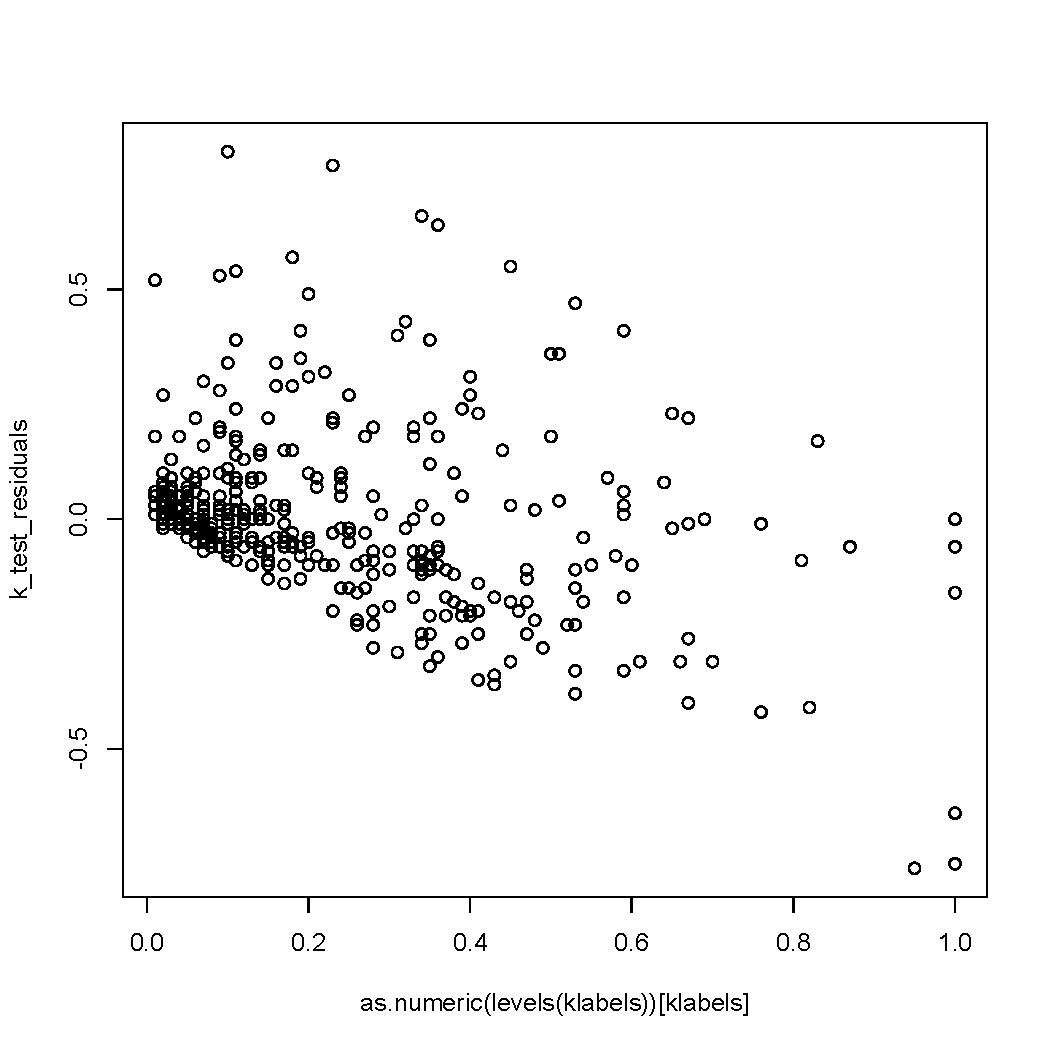
\includegraphics[width=0.7\textwidth,trim= 0 0 20 30, clip]{NN_regression_residuals.pdf}
\end{figure}
\FloatBarrier


\subsection{Conclusions}
The Mean-squared error on k-nearest neighbor \emph{regression} did not work as well as the linear \emph{regression}. Its Mean-squared error was signicantly higher and the \texttt{Residuals Vs Label} plot looks the worse. Scaling the data changed nothing, so we guess that the data set was prescaled.

\newpage
\section{Dealing with missing values}
\subsection{Implementation}

\lstinputlisting[firstline=114, lastline=163]{crimes.R}


\subsection{Results}
\begin{itemize}
    \item Linear Regression (imputed missing values):
    \begin{itemize}
        \item Mean-squared error on the \emph{test data} (20\%): \textbf{1.88e-02}
    \end{itemize}
    \item Nearest Neighbours (imputed missing values):
    \begin{itemize}
        \item Mean-squared error on the \emph{test data} (20\%): \textbf{1.00e-01}
    \end{itemize}
\end{itemize}

\subsubsection{Linear regression}
\vspace{-0.5cm}
\begin{figure}[h!]
    \centering
    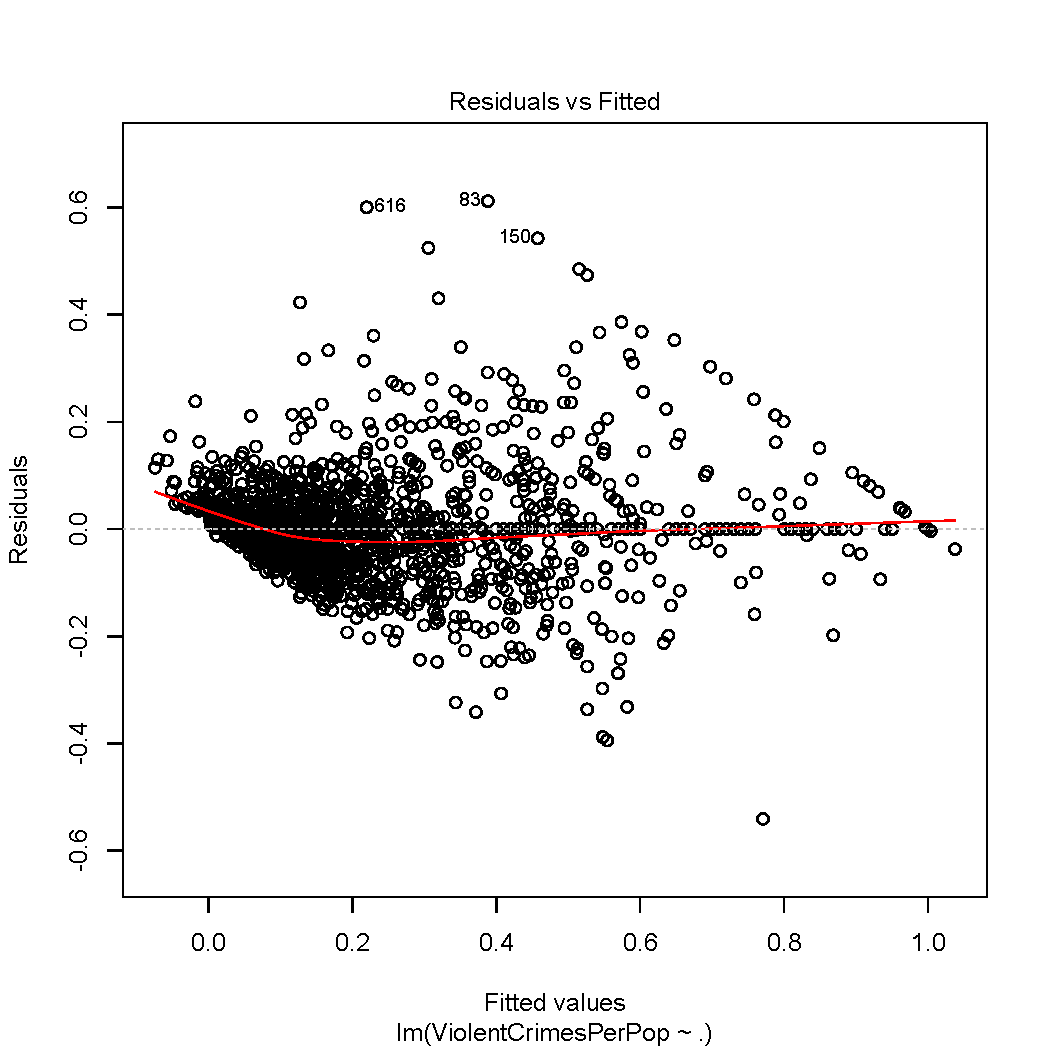
\includegraphics[width=0.7\textwidth,trim= 0 0 20 30, clip]{Unk_linear_regression_residuals.pdf}
\end{figure}
\FloatBarrier

\vspace{-0.5cm}
\begin{figure}[h!]
    \centering
    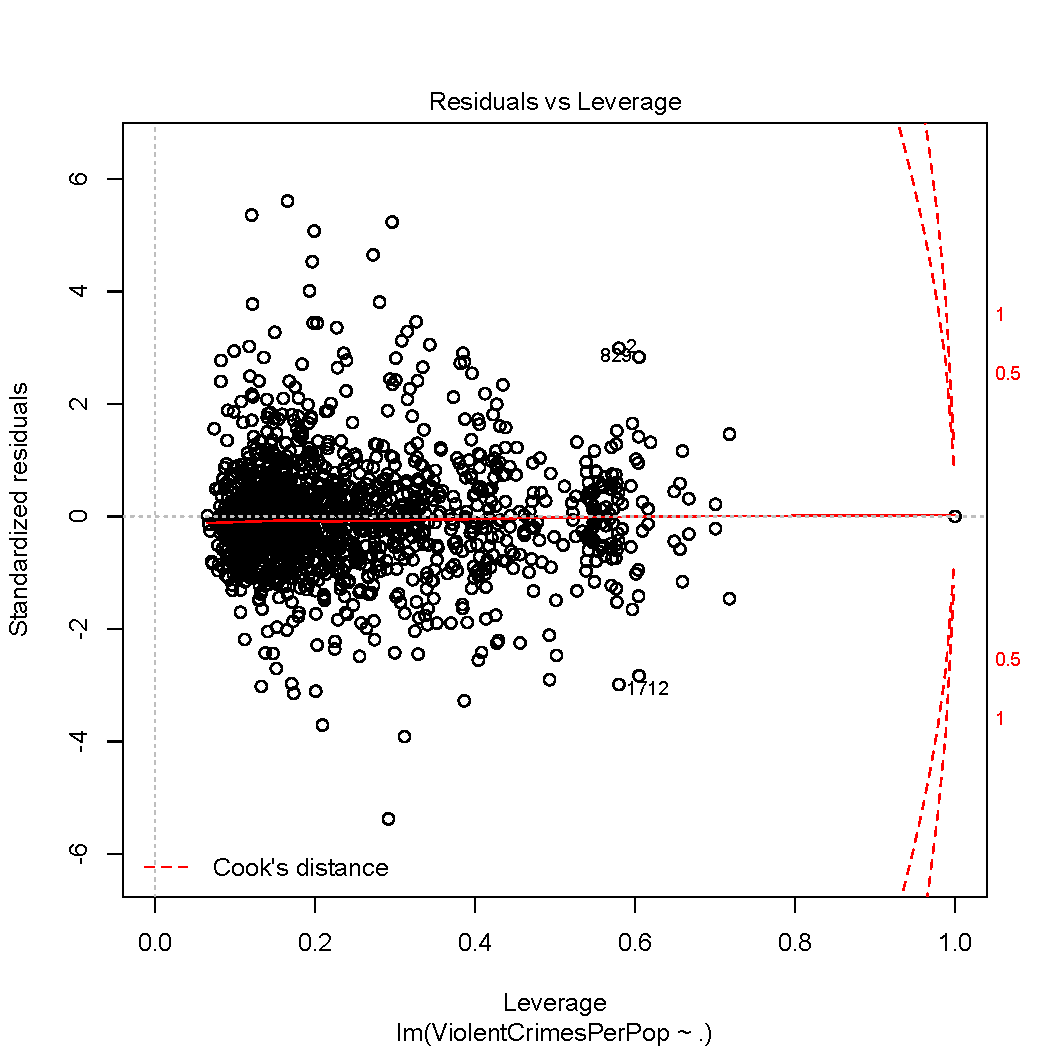
\includegraphics[width=0.7\textwidth,trim= 0 0 20 30, clip]{Unk_linear_regression_cook.pdf}
\end{figure}
\FloatBarrier

\newpage
\subsubsection{Nearest Neighbours}
\vspace{-0.5cm}
\begin{figure}[h!]
    \centering
    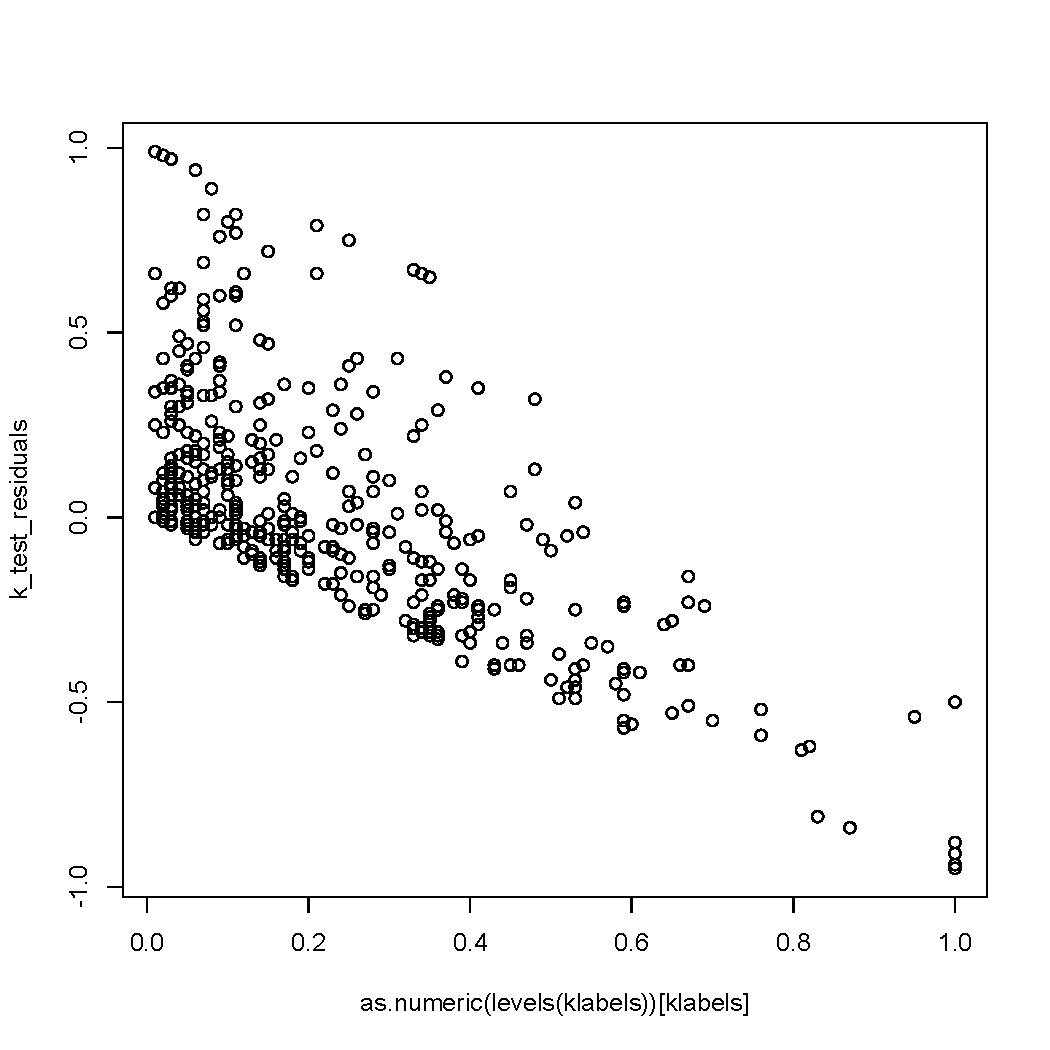
\includegraphics[width=0.7\textwidth,trim= 0 0 20 30, clip]{Unk_NN_regression_residuals.pdf}
\end{figure}
\FloatBarrier

\subsection{Conclusions}
On one side, the Mean-squared error of the test sets did not change much for linear \emph{regression} on this new data with imputed values. On the other side, The Mean-square error was far worse for the nearest neighbors. \\ 

Residuals graph looks like it has a slightly better shape but larger residuals. Also, if you look at the leverage graph it is clear that a few points have higher 
leverage and one point even has a cooks distance of one. \\

It seems that the imputation of missing values let's us have more explanatory variables but it also adds more noise. For linear \emph{regression} it's 
a wash but for nearest neighbors the noise is too much. The additional explanatory variables is not enough to fix our \emph{regression} and are likely not worth the trouble.



\section{Modified Nearest Neighbours}
\subsection{Implementation}
\lstinputlisting{nn-modified.R}

\vspace{-0.4cm}
\subsection{Conclusions}
Two different implementations have been tried for this exercise, one that computes the distance between two vectors with some question mark elements in a linear way (\texttt{distance\_lin}) and other that does the same but with vectorial operations (\texttt{distance\_vec}). \\

Unfortunately, the linear code that uses this distance functions and other \texttt{R} specific instructions to apply the function to matrix columns, like \texttt{outer}, were so slow during the execution that it was impossible to obtain results.

\end{singlespace}
\end{document}
